
\subsection{Charge Asymmetry} \label{sec:chargeasym}

Here, we show our previous results are consistent with
an additional measurement of each photodetector's edge location,
determined by fitting charge asymmetries (Eqn. \ref{eqn:qasym}) between
adjacent photodetectors. 
%This allows for a determination of
%photodetector edges as defined by the midpoint between two detectors,
%in which the X-ray induces charge measurements.

Event selection includes two classes of events; where the X-ray
induced charge is present in one of the channels, or shared by the two
adjacent channels.  The charge selection described in Appendix A
is expanded such that the requirement of minimal charge
can also be satisfied by the sum of charges in the two, adjacently illuminated channels.  
In order to avoid skews to the asymmetry distribution from variation in the gain
of individual photodetectors, the charge from each photodetector is
equalized by the average measured charge in events from the near half of each photodetector.
%The mean
%charge is calculated for each photodetector in the central scanning
%region and normalized before applying selection.

The charge asymmetry for a given set of photodetectors $i,j$
is calculated per event are as  
\begin{equation} \label{eqn:qasym}
    A(Q)  = 
\frac{Q_{i}-Q_{j}}
     {Q_{i}+Q_{j}}, 
\end{equation}
where $i, j$ are chosen to be adjacent photo-detector pairs 
along the direction of the coordinate scanned. The mean value
as a function of the coordinate is fitted to the 
following sigmoid function
\begin{equation}\label{eqn:asymfit}
f_{Asym}(z)=\;
C\,\left[\,Erfc(a(z-z_{0}))-1\,\right],
\end{equation} 
where $z_0$ is the offset in Z, and $C$ and $a$ are 
the scaling parameters of the function.

The center of the asymmetry distribution, $A(Q)=0$ in fig.
\ref{fig:asymplot}, constitutes the physical edge of the
photo-detector -- defined as the midpoint between active regions of the two detectors.  
The photo-detector's position and size are independently calculated in each Z and \phis coordinate as the respective average and separation of the two asymmetry edges.  A
comparison between calculated photo-detector position using X-ray event
rates and charge asymmetry (fig. \ref{fig:asymvsfit}) shows the two
measurements to be consistent.  The photodetector size 
(fig. \ref{fig:mppcsize}) is also in agreement with the
average spacing of the photodetectors previously calculated (table
\ref{tab:avgspacing}).  Due to trigger configuration and the
particular scanning region used in the X-ray survey, photodetectors on
the boundary of trigger region are excluded from the calculation,
limiting this measurement to 15\% of the scanned photodetectors.


\begin{figure}
\centering
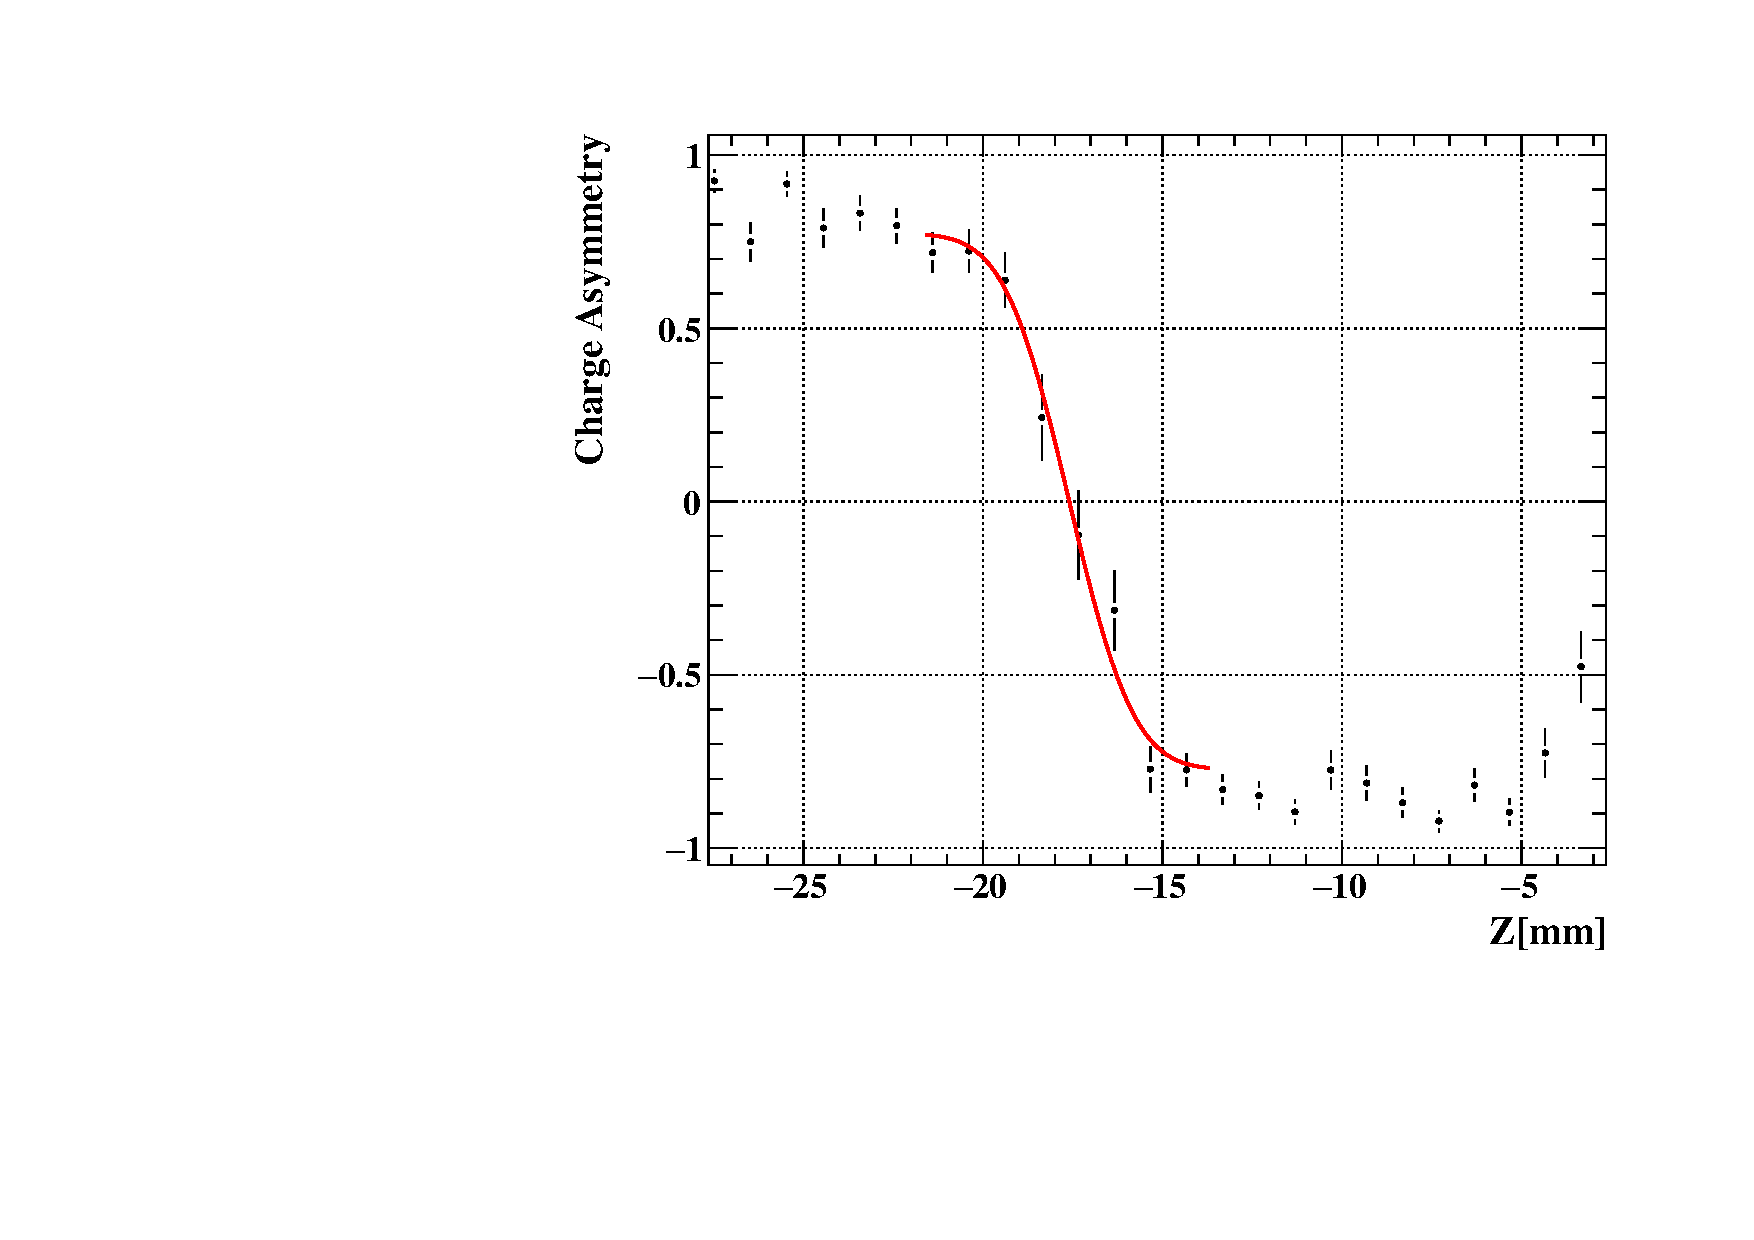
\includegraphics[width=6cm]{graphics/nnasym6465.pdf}
\caption{Mean charge asymmetry calculated as a function of z between 
two photodetectors.}
\label{fig:asymplot} 
\end{figure}

\begin{figure}
\centering
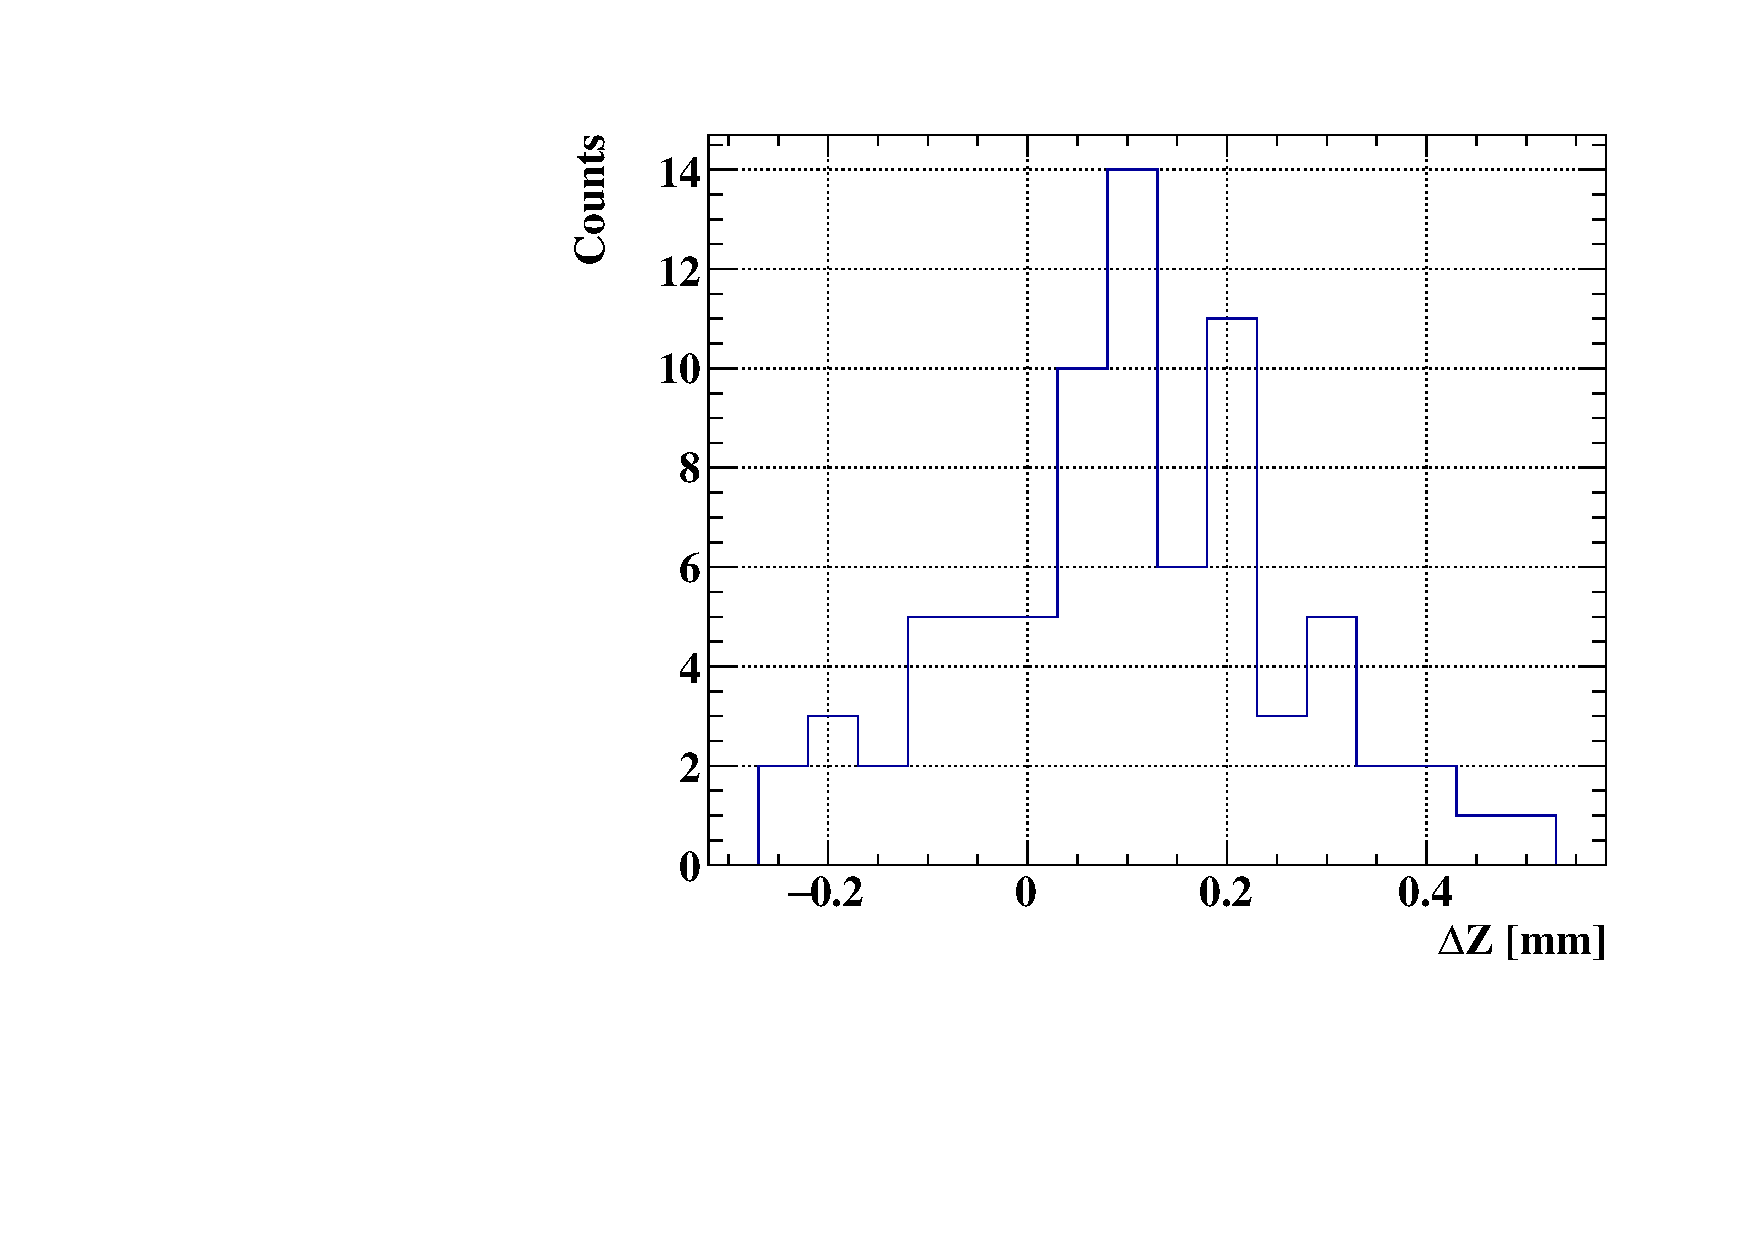
\includegraphics[width=4cm]{asymmetryplots/asymcenterdz.pdf}
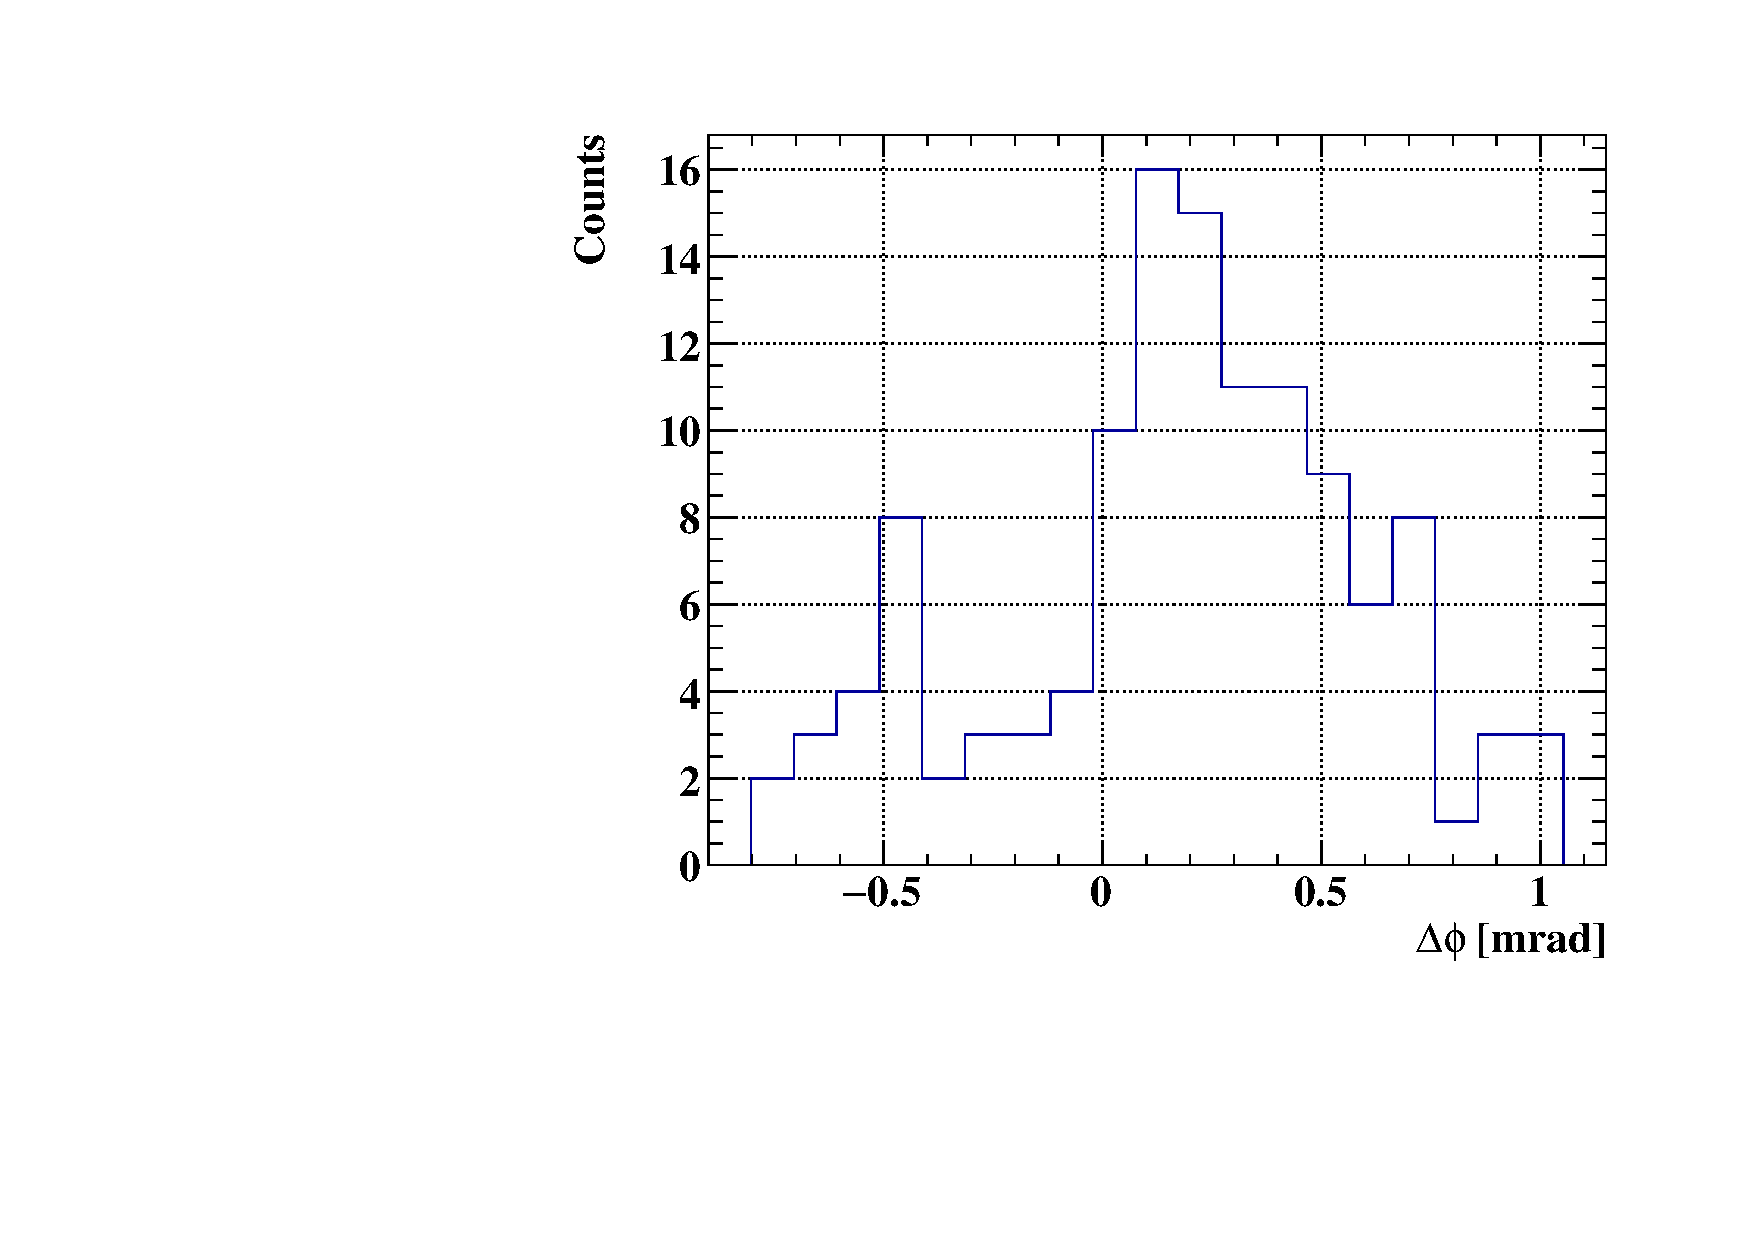
\includegraphics[width=4cm]{asymmetryplots/asymcenterdphi.pdf}
\caption{Comparison between photodetector position calculated from
charge asymmetry and X-ray event rates.}
\label{fig:asymvsfit} 
\end{figure}




\begin{figure}
\centering
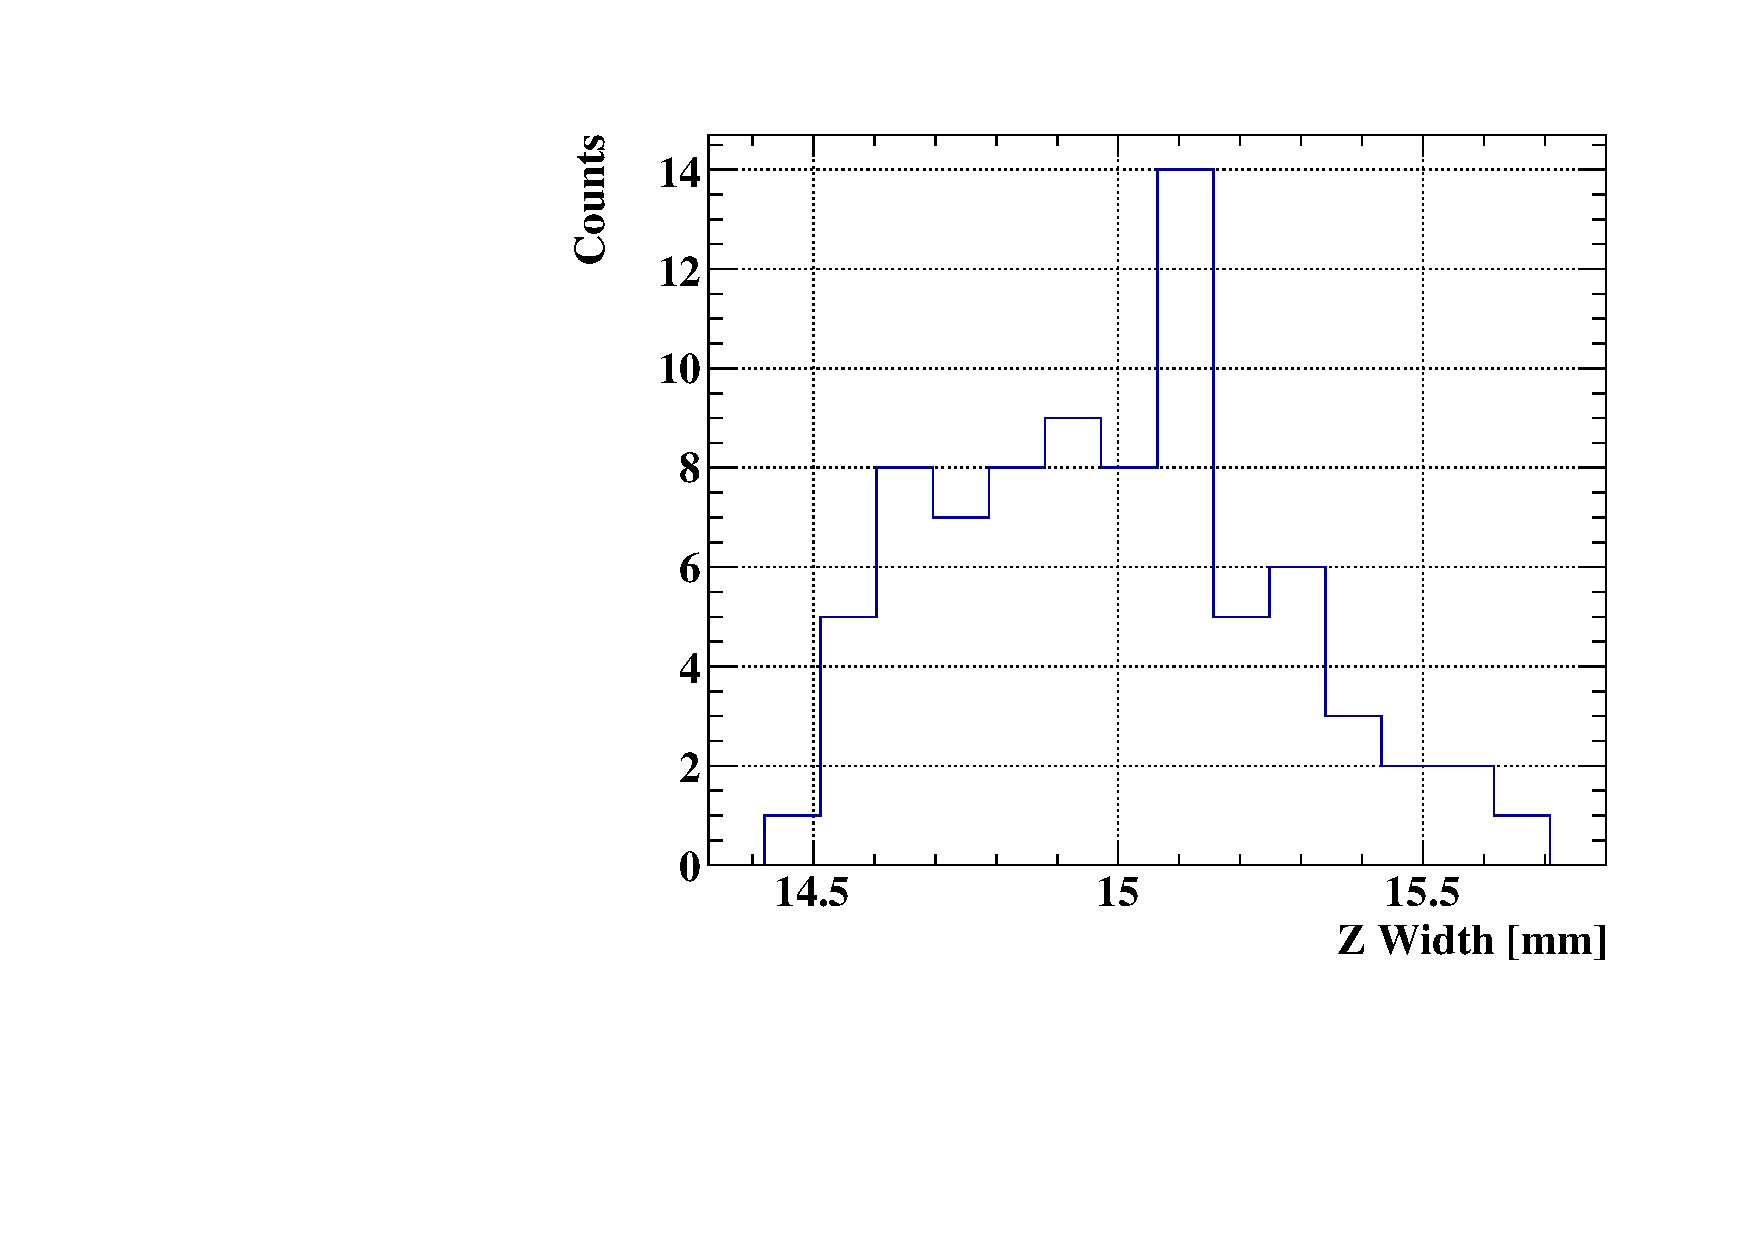
\includegraphics[width=4cm]{asymmetryplots/asymzwidth.pdf}
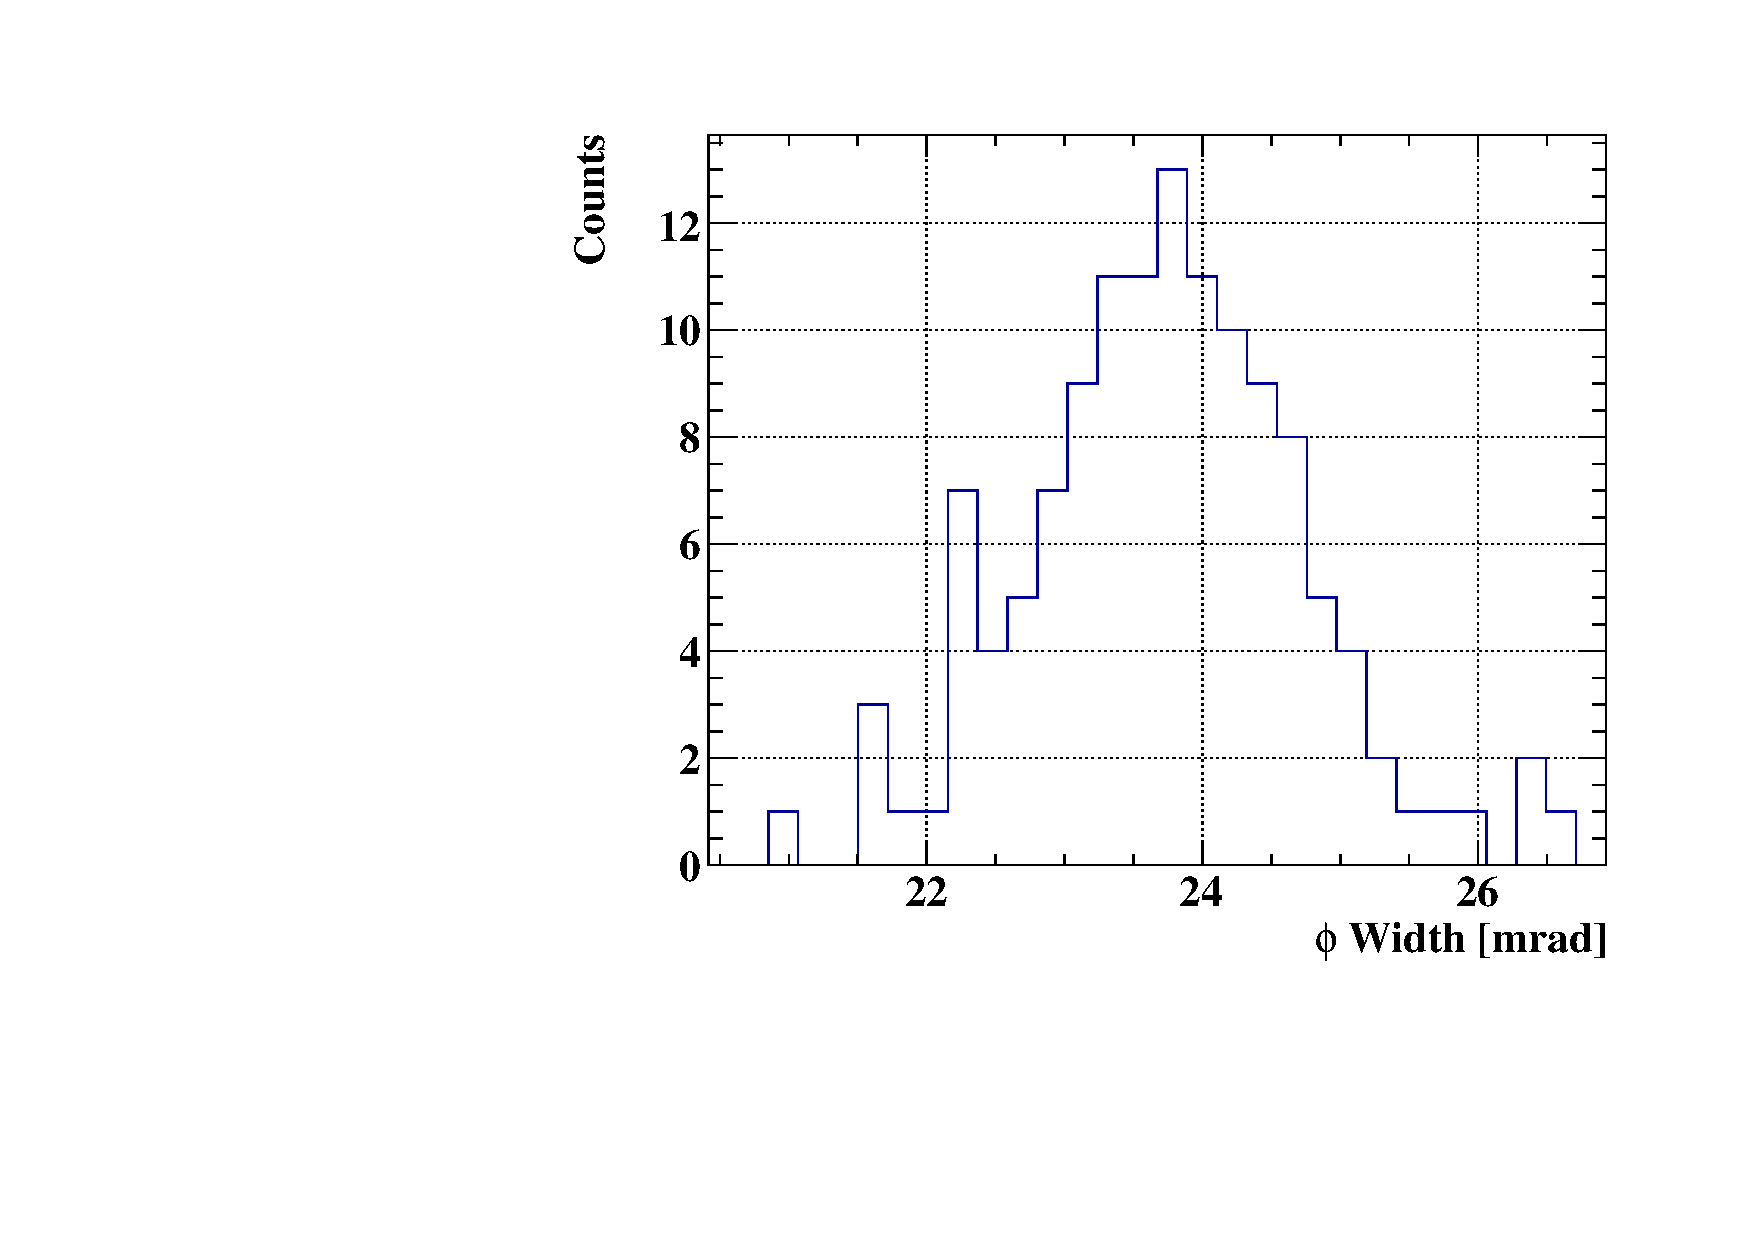
\includegraphics[width=4cm]{asymmetryplots/asymphiwidth.pdf}
\caption{Photodetector size in Z and phi measured using the edge of the
photodetector calculated with charge asymmetry.}
\label{fig:mppcsize} 
\end{figure}

